\documentclass[%
aip,
amsmath,amssymb,
reprint,%
% Conference Proceedings
]{revtex4-1}

\usepackage{graphicx}% Include figure files
\usepackage{dcolumn}% Align table columns on decimal point
\usepackage{bm}% bold math

\usepackage[utf8]{inputenc}
\usepackage[T1]{fontenc}
\usepackage{mathptmx}
\usepackage{graphicx}
\usepackage{array}
\usepackage{listings}
\usepackage{color}

\definecolor{codegreen}{rgb}{0,0.6,0}
\definecolor{codegray}{rgb}{0.5,0.5,0.5}
\definecolor{codepurple}{rgb}{0.58,0,0.82}
\definecolor{backcolour}{rgb}{0.95,0.95,0.92}
 
\lstdefinestyle{mystyle}{
    backgroundcolor=\color{backcolour},   
    commentstyle=\color{codegreen},
    keywordstyle=\color{magenta},
    numberstyle=\tiny\color{codegray},
    stringstyle=\color{codepurple},
    basicstyle=\footnotesize,
    breakatwhitespace=false,         
    breaklines=true,                 
    captionpos=b,                    
    keepspaces=true,                 
    numbers=left,                    
    numbersep=5pt,                  
    showspaces=false,                
    showstringspaces=false,
    showtabs=false,                  
    tabsize=2
}
\lstset{style=mystyle}


\begin{document}

\title{Detecting Expolanets using Unsupervised Deep Learning}

\author{Naveen Mathew Nathan Sathiyanathan}
\affiliation{Department of Statistics, University of Illinois at Urbana-Champaign}

\date{\today}

\begin{abstract}
Exoplanet detection using transit method is currently a manual process. It involves identification of clear troughs in the intensity of light for a sustained period. 
\end{abstract}

\maketitle

\section{Introduction}

Give some introduction

\section{Literature Survey}

Talk about paper which uses CNN, which is supervised learning. Also talk about classical methods: BLS, TLS.

\section{Data Description}

Describe Kepler data

\begin{itemize}
	\item Variable: Description.
	\item Next variable: Next description.
\end{itemize}

\section{Exploratory Analysis}

Speak about number of files, number of stars, number of planets, summary of number of planets around each star. Data is noisy. Talk about median subtraction. Talk about missing data. Add plot

\begin{figure}[h!]
	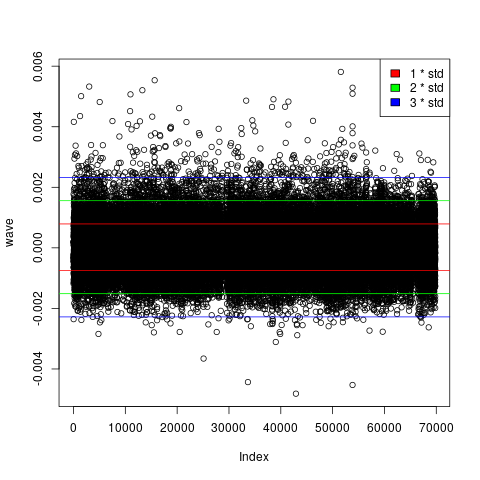
\includegraphics[width=\linewidth]{example.png}
	\caption{Residual Flux vs Time.}
	\label{fig:finaldf}
\end{figure}

Summarize few findings

\section{Preprocessing}

Talk about capping, time series interpolation for filling missing values.

\subsection{Capping}

Something

\subsection{Imputing Missing Values}

Something

\section{Modeling}

Why did you choose the model?

\subsection{Hyper-Parameters}

Some hyperparameters

\section{Results and Conclusions}

Show some good and bad examples. Mention how the results can be improved. Remember, this is completely unsupervised! It can be improved drastically with supervised learning.

\begin{center}
 \begin{tabular}{|c | c | c | c |} 
 \hline
 \textbf{Dataset} & \textbf{Model}& \textbf{Metric} & \textbf{Value} \\ [0.5 ex]
 \hline
 Test & Logistic Regression & AUC & 0.504 \\ 
 \hline
 Test & Logistic Regression & Accuracy & 0.535 \\
 \hline
 Test & Random Forest & AUC & 0.797 \\
 \hline
 Test & Random Forest & Accuracy & 0.73 \\
 \hline
 Test & Stacked Ensemble & AUC & 0.881 \\
 \hline
 Test & Stacked Ensemble & Accuracy & 0.779 \\ [1ex] 
 \hline
\end{tabular}
\end{center}

\vspace{60 mm}
\section*{Appendix}

\begin{itemize}
\item Model building
\end{itemize}

\lstinputlisting[language=R, firstline=10, lastline=20]{"../main.R"}

\begin{itemize}
\item Preprocessing. 
\end{itemize}

\lstinputlisting[language=R, firstline=24, lastline=44]{"../main.R"}

\begin{itemize}
\item The Data Source\\
https://exoplanetarchive.ipac.caltech.edu/bulk_data_download/Kepler_KOI_DV_wget.bat
\item References \\
Identifying Exoplanets with Deep Learning: A Five Planet Resonant Chain around Kepler-80 and an Eighth Planet around Kepler-90 (Christopher J. Shallue, Andrew Vanderburg)\\
Machine-learning Approaches to Exoplanet Transit Detection and Candidate Validation in Wide-field Ground-based Surveys (Schanche et al.)\\

Advances in Financial Machine Learning by Marcos Lopez de Prado

\item Text Sources:
	\begin{itemize}
		\item CNBC
		\item BBC
		\item The Verge
		\item Guardian
		\item Bloomberg
		\item Coindesk
	\end{itemize}
\end{itemize}


\end{document}
















